\cotefile{156-9}
\scanpage{98}\mspage{94}
l'\unsure{ens|ens.} des \deleted{applications} correspondances entre $E,E'$
\[
 \alpha:\unsure{E|{\mathbb E}}\unsure{\mbox{---}|\longrightarrow}
 \deleted{\Sigma_{E'}\unsure{\subset|\in}}\unsure{\mathcal P|\mathscr P|P}(E')
\]
ayant les propriétés

a) $\forall x\in E,\quad\alpha(x)\in\Sigma_{E'}$

b) $\alpha$ satisfait \deleted{\unsure{aux co la con|à une co la con}} conditions équivalentes de la \unsure{propo|prop.} 4, dont la plus explicite est \deleted{\unsure{que que|que expr}} (iv), \deleted{\unsure{qui exprime|qu'exprime}}

Soit enfin
\[
 \operatorname{Corr}^{\unsure{\times|\star|\kappa}}(\underline E,\underline{E'})
\]
l'ensemble des \deleted{applications \unsure{parties|partielles}}\inserted{corr. ensemblistes $R$} entre \deleted{$\alpha^{\times}:E\unsure{\mbox{---}|\longrightarrow}\mathcal P(E')$} $E$ et $E'$ $(R\subset E\times E')$ telles que
\[
 \left\{\begin{aligned}
 &\forall x\in E,\quad R(x)\in\Sigma_{E'}\\
 &\forall x'\in E',\quad {}^{t}R(x')\in\Sigma_E\;.
 \end{aligned}\right.
\]

On a \unsure{donc|alors} des \deleted{correspondances}\inserted{\unsure{applications|aplications}} biunivoques canoniques
\diagram{\begin{tikzcd}[ampersand replacement=\&,column sep=large]
 {\operatorname{Corr}(\unsure{\Sigma|{}^{t}\Sigma},\Sigma')} \arrow[r,"{\substack{\varphi\\[-.3ex]\sim}}"] \&
 {\operatorname{Corr}(\underline E,\underline{E'})} \arrow[r,"{\substack{\psi\\[-.3ex]\sim}}"] \&
 {\underline{\operatorname{Corr}}^{\times}(\underline E,\underline{E'})}
\end{tikzcd}}
\unsure{Obtenues|Obtenus} ainsi :
\[
 \left\{\begin{aligned}
 &\varphi(\alpha_{*})=\alpha_{*}\circ\sigma_E
 \quad:\quad E\xrightarrow{\sigma_E}\Sigma_E\xrightarrow{\unsure{\alpha_{\times}|\alpha_{*}}}\Sigma_{E'}\\
 &\psi(\alpha)=\bigl\{(x,x')\deleted{\}}\in E\times E'\bigm|
 \alpha(x)\mathrel{|\,\unsure{\circ|o|0}\,|}x'\quad
 \text{\unsure{i.e|ie}}\quad x'\in\operatorname{cosupp}^{\unsure{\bullet|\circ}}_{E'}(\alpha(\unsure{x)|x|x))\}}
 \end{aligned}\right.
\]

(Ainsi $\psi(\alpha)$ n'est pas le graphe de la correspondance $\alpha:E\longrightarrow\deleted{\mathcal P(E')}\inserted{\Sigma_{E'}\subset}\mathcal P(E')$, mais de la correspondance \unsure{déduite} en composant avec $\unsure{\complement|C}_{\Sigma'}\quad E\xrightarrow{\alpha}\Sigma_{E'}\xrightarrow{\complement_{E'}}\Sigma_{E'}\subset\mathcal P(E')$)
% archive sheet number: 97
\scanpage{99}\mspage{95}
Il reste seulement à prouver que si $\alpha_{*}$ est dans $\operatorname{Corr}(\Sigma,\Sigma')$, alors $\alpha=\varphi(\alpha_{\unsure{\times|*}})$ satisfait aux conditions de \unsure{propo|prop.} 4\unsure{,} et \unsure{redonne} $\alpha_{*}$, par
\[
 \alpha_{*}(S)=\mathop{\mathrm{Sup}}\limits_{x\in S}{}_{\Sigma_{E'}}
 \underset{\inserted{\substack{\Vert\,\text{\unsure{def.|déf.}}\\
 \alpha_{*}^{\unsure{\cdot|\prime}}(\operatorname{supp}^{\unsure{\bullet|\circ}}_E(x))}}}{\underline{\alpha(x)}}
 \qquad(S\in\Sigma_E)\unsure{,|.}
\]
\deleted{Ce qui}\inserted{Cette formule} provient de la formule
\[
 S=\mathop{\mathrm{Sup}}\limits_{x\in S}{\unsure{\operatorname{supp}|\deleted{\operatorname{supp}}\sigma}}^{\bullet}_E(x)
\]
et de la commutation de $\alpha_{*}$ avec $\mathrm{Sup}$.

Ainsi, il reste à prouver (iv b) sur $\alpha$ :
\[
 \bar\alpha(\deleted{\operatorname{supp}}\inserted{\sigma}^{\unsure{\bullet|\circ}}_E(x))\deleted{\unsure{\in|{=}}}
 \text{ et }\alpha(x)\quad\text{ont }=\operatorname{supp}^{\bullet}_{E'}\,.
\]
Or si $y\in\deleted{\unsure{\operatorname{supp}|\Sigma}}\sigma_E(x)$, on a
$\deleted{\operatorname{supp}^{\bullet}_E(y)\leq\operatorname{supp}^{\bullet}_E(x)}\inserted{\sigma_E(y)\leq\sigma_E(x)}$
d'où $\deleted{\alpha_{*}\unsure{(|\in}}\underset{\deleted{\alpha(y)}}{\underline{\alpha_{*}\,\sigma_E(y)}}\leq\alpha_{*}\,\sigma_E(x)\quad\text{i.e.}\quad\underset{\inserted{\text{dans }\Sigma_{E'}}}{\underline{\alpha(y)\leq\alpha(x)}}$,
donc \deleted{\unsure{les|le} $\bar\alpha$}
\[
 \operatorname{supp}^{\bullet}_{E'}\bigl(\bar\alpha(\sigma_E(x))\bigr)\leq
 \deleted{\text{\unsure{ont même|ont}}\quad
 \unsure{\sum_{T\leq\alpha(x)}|\Sigma_{T\leq\alpha(x)}}\quad
 \text{\unsure{de|et}}\quad\operatorname{supp}^{\bullet}_{E'}}\,\alpha(x)
\]
\deleted{\unsure{du|de}} $\deleted{\alpha_{*}(\sigma_E(x))}$
\[
 \deleted{\bar\alpha(\sigma_E(x))\quad\text{et}\quad\alpha(x)}
 \qquad\text{\unsure{qed.|Qed.}}
\]
\figure{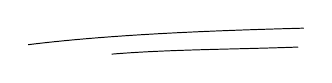
\begin{tikzpicture}[x=1cm,y=1cm]
\draw[line width=.35pt] (0,0) .. controls (1.05,.13) and (2.35,.18) .. (3.5,.21);
\draw[line width=.35pt] (1.06,-.12) .. controls (1.78,-.06) and (2.60,-.06) .. (3.43,-.03);
\end{tikzpicture}}

\margin{\unsure{11.7.|II.7.}}On va faire une \uline{\unsure{categorie|catégorie}} avec les \unsure{disjoncteurs|disponcteurs}, en prenant comme morphismes $\underline E_{\unsure{,|\ell|1}}\unsure{\longrightarrow|\mbox{---}}\underline{E'}$ les correspondances qui satisfont a) b) de la page 94 avec la composition (si $\underline E\xrightarrow{\alpha}\underline{E'}\xrightarrow{\beta}\underline{E''}$)
\[
 \beta\underset{\mathrm{dis}}{\circ}\alpha=
 \deleted{\bigl(\beta\underset{\mathrm{ens}}{\circ}\alpha}
 \operatorname{supp}_{E''}^{\bullet}\bigl(\beta\underset{\mathrm{ens}}{\circ}\alpha\bigr).
\]
\unsure{Cette|Cela}
% archive sheet number: 98
\scanpage{100}\mspage{96}
composition est associative, avec \deleted{\unsure{les|des}}\inserted{\unsure{comme|pour}} identités $\deleted{\unsure{\mathrm{id}_{\underline E}|\alpha_{\underline E}}}\sigma_{\underline E}=\operatorname{supp}^{\unsure{\circ|\bullet}}_{\underline E}\circ\mathrm{id}_{\unsure{E|\underline E}}$. La catégorie des \unsure{disjoncteurs|disponcteurs|disponteurs} et correspondances \deleted{\unsure{de|des}}\inserted{entre} \unsure{telles|icelles|elles}, est \unsure{équivalente} à la catégorie des disjoncteurs canoniques ou \unsure{spatios} (ou ``\uline{\unsure{espaceurs}}'' ?), \unsure{ou|où} on prend comme morphismes les \uline{applications} \unsure{croissantes} qui commutent aux sup quelconques\inserted{(appelées encore ``correspondances'' entre les spatios)}. Et cette catégorie est canoniquement équivalente à la catégorie opposée, par une ``autodualité'' (involutive) qui est l'identité sur les objets, et sur les morphismes est le passage à la \unsure{flèche|flèches} transposée\unsure{.|..}

[Analogie avec les espaces de Hilbert, ou \inserted{plus \unsure{gén.|gén}} espaces vectoriels munis d'une autodualité\ldots, et les opérateurs adjoints\ldots]

\margin{\figure{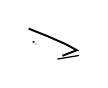
\begin{tikzpicture}[x=1em,y=1em]
 \draw[line width=.7pt] (0,1.1) -- (.7,.82) -- (1.36,.53) -- (1.74,.32) -- (1.22,.12);
 \draw[line width=.45pt] (1.04,0) -- (1.82,.13);
 \fill (.18,.62) ellipse (.055 and .03);
 \fill (.27,.54) circle (.022);
\end{tikzpicture}}}\uline{Questions ouvertes}, que je ne vois pas moyen de tirer au clair, \unsure{suggérées} par le cas des disjoncteurs triviaux.
% archive sheet number: 99
\scanpage{101}\mspage{97}
Dans ce cas les correspondances \unsure{de|des} \unsure{disjoncteurs|disponcteurs} sont les corr. ensemblistes, elles forment l'ensemble $\unsure{\mathcal P|\mathscr P|P}(E\times E')$, qui est lui-même un \deleted{disjoncteur} \unsure{spacios|spatios}, associé au disjoncteur trivial $E\times E'$. Il serait \unsure{tentant} alors, dans le cas général, de vouloir interpréter les correspondances de disjoncteurs \inserted{de $\underline E$ à $\underline{E'}$} comme étant les éléments du spatios associé au ``disjoncteur produit'' $E\times E'$, avec
\[
 (x,x')\mathrel{|\,\unsure{\supset|\circ|o|0}\,|}(y,y')
 \overset{\text{\unsure{def|déf}}}{\Longleftrightarrow}
 x\mathrel{|\,\circ\,|}x'\quad\text{\uline{ou}}\quad y\mathrel{|\,\circ\,|}y'.
\]

On vérifie en effet que les \deleted{supports} $R\in\Sigma_{E\times E'}$ sont dans l'ens. noté $\operatorname{Corr}^{\unsure{\times|\star|\kappa}}(\underline E,E')$ (p. 94) i.e. $\deleted{\unsure{R|\mathcal R}}\forall \deleted{\unsure{\alpha|x}}x\in E,\ R(x)\in\Sigma_{E'}^{\unsure{7|\urcorner|\prime|?}}$, et $\forall x'\in E',\ {}^{t}R(x')\in\Sigma_E$. Mais il ne semble pas que \deleted{\unsure{tout|tait}} l'inverse soit vrai, \unsure{\uline{sauf}|sauf} dans le cas où $\underline E$ \uline{ou} $\underline{E'}$ est \deleted{\unsure{le|l'}}un disjoncteur trivial.

Mais si ce n'était pas vrai en général, la question demeure si l'ens. des \deleted{\unsure{disjo|dispo}} corr. de $\underline E$ à $\underline{E'}$, ou \inserted{encore} des \deleted{\unsure{morphismes}}\inserted{\unsure{corr..|corr.}} de spatios $\Sigma\unsure{\mbox{---}|\longrightarrow}\Sigma'$, forme un spatios. La relation d'ordre suggérée par le cas \unsure{d'ensembliste|ensembliste} (disj. triviaux) est simplement
% archive sheet number: 100
\scanpage{102}\mspage{98}
\[
 f\leq g\quad\overset{\text{\unsure{dfn|defn|def}}}{\Longleftrightarrow}\quad
 \forall x\in\Sigma,\qquad f(x)\leq g(x)\;.
\]

\unsure{Je|J} dis que pour cette relation d'ordre dans $\operatorname{Corr}(\Sigma,\Sigma')$, les $\mathrm{Sup}$ quelconques (donc aussi les $\mathrm{Inf}$ quelconques) existent, et sont \unsure{données|donnés} par
\[
 \bigl(\mathop{\mathrm{Sup}}\limits_i \unsure{f^{\cdot}|f_i|f'}\bigr)(x)
 =\mathop{\mathrm{Sup}}\limits_i \unsure{f^{\prime}|f^{\cdot}|f_i}(x)\qquad\forall \unsure{x|\cdot}\in\Sigma.
\]
En effet, l'associativité des $\mathrm{Sup}$ montre que l'application du second \unsure{mb|=b} commute bien aux $\mathrm{Sup}$ \unsure{quelc.|quelc}, donc est une corr. de spatios.

Mais la structure $C$, ou la structure de \unsure{disjonction|disponction}, n'est pas claire.

Dans le cas où $E$ est un \unsure{disjoncteur|disponcteur} trivial, \deleted{on a \unsure{une}} et où les corr. $E\unsure{\mbox{---}|\longrightarrow}\Sigma'$ sont \inserted{\unsure{données par}} les applications quelconques $\deleted{\Sigma}E\unsure{\mbox{---}|\longrightarrow}\Sigma'$, donc
\[
 \operatorname{Corr}(\deleted{E}\Sigma_E,\Sigma')\simeq{\Sigma'}^{E},
\]
les structures de disjonction et $C$ peuvent \unsure{de|se} décrire ``terme par \unsure{terme|termes}''
\[
 (\unsure{\complement|C} f)(x)=\complement f(x)\qquad\forall x\in E
\]
% archive sheet number: 101
\scanpage{103}\mspage{99}
\[
 f\mathrel{|\,\unsure{\circ|o|0}\,|}g\quad\Longleftrightarrow\quad
 \forall x\in E,\qquad f(x)\mathrel{|\,\unsure{\cdot|\circ|o|0}\,|}g(x)
\]
mais si on prend des arguments dans $\unsure{\mathcal P|\mathscr P|P}(E)$ et non dans $E$, on n'a bien sûr \deleted{plus} en \unsure{général|générale}
\[
 \left.\begin{aligned}
 &(\unsure{\complement|C}\unsure{f|d})(A)\ne\complement(f(\unsure{A|A'|\Lambda'|x}))\\
 \text{et}\quad &f\mathrel{|\,\circ\,|}g\quad\nRightarrow\quad f(A)\mathrel{|\,\circ\,|}g(A)
 \end{aligned}\ \right|\quad A\in\deleted{\unsure{\mathcal P|E}}\Sigma_E=\mathcal P(E)
\]

On voit donc que la question de définir $C$ ou $\mathrel{|\,\circ\,|}$ sur $\operatorname{Corr}(\Sigma,\Sigma')$ en général, semble \unsure{lié|liée} à la question \unsure{de'|d'}arriver à mettre le doigt, \deleted{soit} sur des éléments minimaux de $\Sigma\setminus\{0_{\Sigma}\}$, ou d'autres objets mathématiques qui en tiendraient lieu, jouant le \unsure{rôle|role} \unsure{de|des} ``points''.

Une question sans doute étroitement \unsure{apparentée} est la suivante. Dans le cas ensembliste (disj. triviaux), \unsure{utilisant} le graphe $\Gamma\inserted{\subset E\times E'}$ d'une correspondance, \deleted{celle-ci peut}
% archive sheet number: 102
\scanpage{104}
\mspage{100}

\diagram{\begin{tikzcd}[ampersand replacement=\&]
\Gamma \arrow[r,"{f'}"{anchor=base,inner sep=0pt}] \arrow[d,"f"'] \& E'\\
E \&
\end{tikzcd}}

celle-ci peut se décomposer en
\[
\Gamma=f'\circ{}^{t}f,
\]
i.e. ``l'inverse'' d'une application'' 
\[
\begin{aligned}
\text{(donnant lieu \unsure{:|à}} &\quad A\mapsto f^{-1}(A),\qquad\text{)}\\
&\quad \unsure{\mathcal P|\mathscr P|P}(E)\mathrel{\unsure{-|\to}}\mathcal P(\Gamma)
\end{aligned}
\]
\unsure{suivi|suivie} de l'application $f'$ (donnant lieu :
\[
B\mathrel{\unsure{-|\mapsto|\to}}f'(B),\quad
\mathcal P(\Gamma)\mathrel{-}\mathcal P(E')\text{).}
\]

Une corr. de la forme $ {}^{t}f$ \deleted{\unsure{peut d'|peut d}} (``comorphisme'') peut d'ailleurs se caractériser\unsure{.} \inserted{algébriquement en termes de corr. de \unsure{spatios|Spatios},} par la propriété de \unsure{commutation} à $C$; \deleted{e}Et \unsure{dualement|dualemt}, une correspondance de la forme $f'$ (``morphisme'') se caractérise par la propriété que \unsure{son|sa} transposé $ {}^{t}f'$ commute à $C$.

Y-a-t-il une décomposition similaire dans le cas général des \unsure{corresp|corr.} \deleted{\unsure{de|des}} entre \unsure{disjoncteurs|disponcteurs}, ou ce qui revient au même, entre spatios ?
% archive sheet number: 103
